\chapter{Model predictive control}
\section{Optimal control problem}
	The optimal control problem goes back more than 300 years. From Galileo and Newton to Johann Bernoulli and Euler with the Brachistochrone problem. The goal in optimal control is to find the appropriate inputs or control law, so that the dynamic system behaves optimally, according to some criterion. 
	
	The main ingredients involved in the definition of an optimal control problem are: a set of differential equations that describes the behavior of the system. A cost function that describes the cost of the specific trajectory integrated on the differential equations.
	
	Optimal control problems can be mathematically defined as \eqref{eq:optimal control definition}.
	
	\begin{subequations}\label{eq:optimal control definition}
		\begin{alignat}{4}
		\min_u \ & \int_{t_0}^{T} L[x(t),u(t),t] \label{eq:optimal control definition cost}\\ 
		\text{subject to: } & \dot{x}(t) = F(x(t),u(t),t) \label{eq:optimal control definition system}\\
		& B[x(t_0),t_0,x(T),T]=0  \label{eq:optimal control definition boundary condition}\\
		& C[x(t),u(t),t]\le 0  \label{eq:optimal control definition constraints}
		\end{alignat}
	\end{subequations}
	
	Equation~\ref{eq:optimal control definition boundary condition} represents the boundary conditions, the behavior of the system is described in equation~\ref{eq:optimal control definition system}. Additionally equation~\ref{eq:optimal control definition constraints} represents constraints on the state and input.

\section{MPC}
	Model predictive control is an advanced control method that continuously solves an  optimal control problem in real-time. At a constant rate the state is measured, an optimal control problem is defined and solved. The optimal input as in the first input of horizon is applied to the system, and the cycle repeats itself.
	
	A continuous-time physical system can be defined as $\dot{x}=F_c(x,u)$, where $x$ is the current state and $u$ is the current input. However when using computer systems it is often required to have a discrete-time system. A discrete integrator can transform a continuous-time system into a discrete-time system, defined as: $x^{k+1}=F_d(x^{k},u^{k})$. 
	
	Figure~\ref{fig:MPC diagram} is a diagram from Wikipedia \cite{Wikipedia} that illustrates MPC. The reference trajectory is the wanted behavior, the predicted control input is the input that is obtained from the controller that leads to the predicted trajectory.
	\begin{figure}[h]
		\centering
		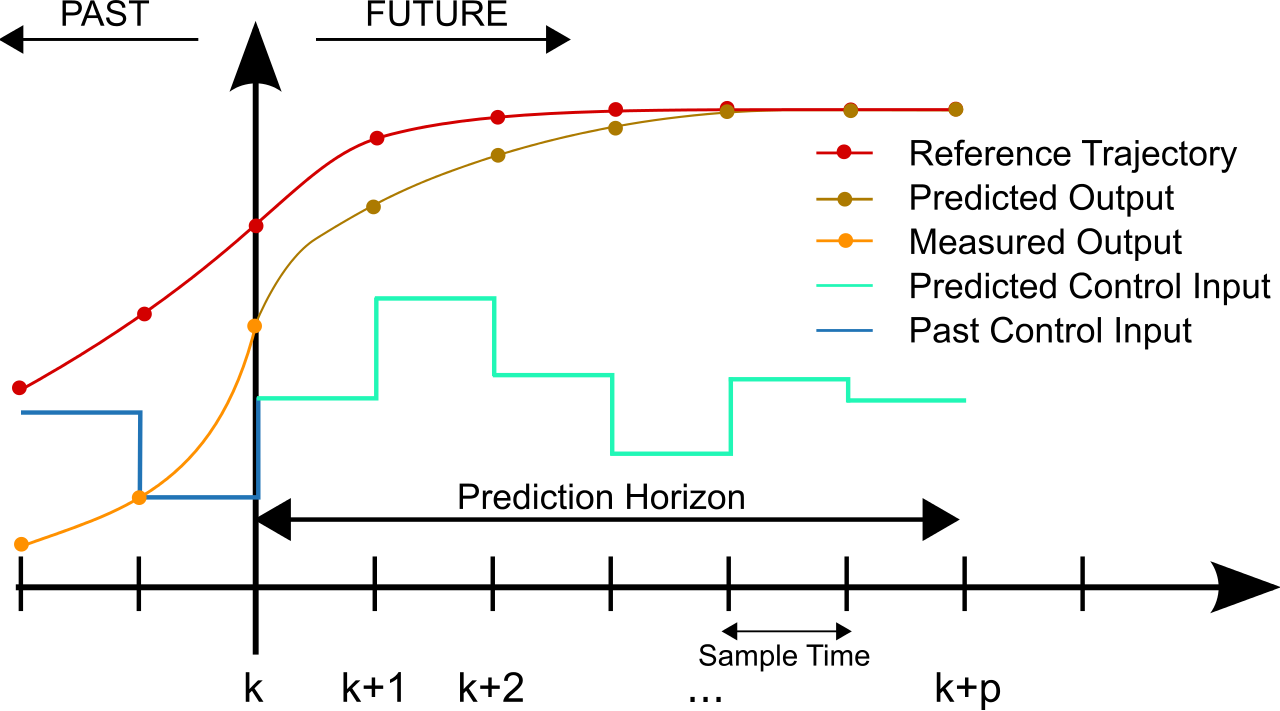
\includegraphics[width=0.7\textwidth]{MPC_scheme}
		\caption{A simple MPC diagram from the wikipedia page \cite{Wikipedia}}
		\label{fig:MPC diagram}
	\end{figure}
			
	\subsection{System}
		
	\subsection{Problem definition}
	The problem definition is based on \cite{Diehl2005}.
		\subsubsection{Problem form}
			The optimal control problem can be written as a non linear programming (NLP) problem  \eqref{eq:PANOC MPC form}. When solved the optimal inputs are obtained for a given initial state $x_0$. \begin{equation}
			\underset{u}{\minimize} \  f(x_0,u) + g(u)
			\label{eq:PANOC MPC form}
			\end{equation}
			
			 Sometimes $x_0$ will be assumed to be part of the function $f$, just like the reference state and reference input, which leads to the simplified equation of \eqref{eq:PANOC form} .
				
			\begin{equation}
				\underset{u}{\minimize} \  f(u) + g(u)
				\label{eq:PANOC form}
			\end{equation}
		\subsubsection{Direct Single shooting}
			The direct single shoot definition with a predict horizon of N, can be written as a NLP that is solved for $u=[u_0,u_1,... u_{N-1}]$. Each of the $u_k$ vectors contains the inputs of the system at a particular time in the predict horizon. This means that the size of the vector $u$ is the predict horizon multiplied by the dimension of the input .
			
			The cost on each step in the horizon is defined as \eqref{eq:single shot iteration cost}, this is called the stage cost.
			\begin{equation}
				\begin{aligned}
				& l_k(x_0,u) = &&  x_k^T Q x_k  +  u_k^T R u_k \\
				& \text{subject to}			&& x_0 = \bar{x} \\
				& 							&&  x_{n+1} = F_d(x_n,u_n), n=0...N-1
				\end{aligned}
				\label{eq:single shot iteration cost}
			\end{equation}
			
			The terminal cost is a special case of the stage cost, it is the last stage cost in the predict horizon. So if the Horizon is N, the terminal cost can be defined as \eqref{eq:single shot terminal cost}.
			
			\begin{equation}
				\begin{aligned}
					& l_N(x_0,u) = && x_N^TSx_N \\
					& \text{subject to}			&& x_0 = \bar{x} \\
					& 							&&  x_{n+1} = F_d(x_n,u_n), n=0...N-1
				\end{aligned}
				\label{eq:single shot terminal cost}
			\end{equation}
			
			So according to \cite{Diehl2005} the cost function $f(x_0,u)$ then becomes \eqref{eq:single shot definition}, the sum of the stage costs and the terminal cost.
			
			\begin{equation}
				f(x_0,u) = \sum_{k=1}^{N-1} l_k(x_0,u) + l_N
				\label{eq:single shot definition}
			\end{equation}
			
			An other term can be added to \eqref{eq:single shot definition} to represent the obstacle avoidance. More on this later in the subsection on obstacles.
		\subsection{Direct Multiple shooting}
			The multiple shoot as defined in \cite{Diehl2005} uses more initial information than just the initial inputs of the predict horizon. It requires an initial estimate of the intermediate states. These state estimates will be referred to as $x_i$ and the states derived from the estimate and its corresponding input will be referred to as $\bar{x_i}$. 
			
			Just as with the Single Shot, the goal is to find the optimal inputs $u_i$. However there are additional continuity conditions: $\bar{x_i} - x_{i+1} = 0$.
			
			\begin{equation}
				\bar{x_i} = F(x_i,u_i)
				\label{eq:}
			\end{equation}
			
			The continuity conditions are displayed in \eqref{eq:continuety condition multiple shot} and were not necessary with the single shot definition, as there are no state estimates. If the initial state estimates are relatively close to the solution, a significant speed increase can be accomplished.
			
			\begin{equation}
				\bar{x_i} - x_{i+1} = 0
				\label{eq:continuety condition multiple shot}
			\end{equation}
			
			The direct multiple shoot definition is formally defined as \eqref{eq:multiple shot cost} in \cite{Diehl2005}, and has an extra equality condition compared to the single shoot. The continuity conditions can be added as a soft constraints to the cost function. This leads to \eqref{eq:multiple shot cost with soft constraint} and can be used with PANOC.
			
			\begin{equation}
				L = \sum_{i=1}^{N} l(\bar{x_i},u_i) \\
				\label{eq:multiple shot cost}
			\end{equation}
			
			\begin{equation}
			L =  \sum_{i=1}^{N} l(\bar{x_i},u) + c \cdot ||\bar{x_i} - x_{i+1}||^2
			\label{eq:multiple shot cost with soft constraint}
			\end{equation}
			
			The simulation results of multiple shoot with the PANOC algorithm are quiet bad and not further discussed. However it might be interesting to revisit this subject when the Lagrangian is introduced later on.
		\subsection{Obstacle avoidance}
			It is often required to avoid certain states or inputs. the states that must be avoided will be called obstacles. One way to add these obstacles to the problem is via a soft constraints on the cost function. This means that these cost functions must be twice differentiable.\cite{AjaySathya2017} Describes these obstacles as either a set of unwanted states or non-linear constraints on the states.
			
			\subsubsection{As set}
				 The obstacle can be defined as a bounded set, as illustrated by \eqref{eq:obstacle as open set}. It is determined by the intersection of a set of non-linear inequalities.
				\begin{equation}
					O = \{ z \in \Re^{n_d} : h^i(z)>0,\ i \in N_{[1,m]} \}
					\label{eq:obstacle as open set}
				\end{equation}
				Where $ h^i:\Re^{n_d} \rightarrow \Re $ are $C^{1,1}$ functions.
				
			\subsubsection{As constraint}
				\begin{equation}
					[z]_+ =  \max\{0,z\}
				\end{equation}
				
				The statement $h(x)<0$ is equivalent to stating $[h(x)]_+=0$, so \eqref{eq:obstacle as open set} is equivalent to setting \eqref{eq:obstacle as equality} to zero.
				
				\begin{equation}
					\Phi_0(z) =  \frac{1}{2} \prod_{i=1}^m \Big( [h^i(z)]_+ \Big)^2
					\label{eq:obstacle as equality}
				\end{equation}
				
				The gradient of \eqref{eq:obstacle as equality} is define as \eqref{eq:obstacle as equality} in \cite{AjaySathya2017}.
				
				\begin{equation}
					\nabla \Phi =
					\begin{cases}
						\sum_{i=1}^{m} h^i(z)\prod_{j \ne i} \Big( [h^j(z)]_+ \Big)^2 \nabla h^i(z)
						& x \in O \\
						0 & else
					\end{cases}
					\label{eq:derivative obstacle as equality}
				\end{equation}
			
			\subsubsection{Polyhedral obstacle}
				A simple obstacle example of such an obstacle is a polyhedral as defined in \eqref{eq:polyhedral constraint}.
				\begin{equation}
					\prod \Big([b_i - a_i^t z]_+ \Big)^2 = 0
					\label{eq:polyhedral constraint}
				\end{equation}
			
			\subsubsection{Obstacle as soft constraint}
				The obstacle avoidance is added as a soft constraint into the cost function. As demonstrated in \eqref{eq:derivative obstacle as equality}, this definition is still two times differentiable.
			
		\subsection{Input constraints}
			An other important aspect of a MPC problem is the input constraint. In practice inputs have to comply with the physical properties of the devices. For instance absurdly high or low input values might in theory lead to a fast solution, but are not feasible in practice.
			
			A major advantage of the PANOC algorithm is that it can take non-linear or non-convex constraints. As longs as the proximal mapping is analytically defined it is feasible. 
			
			A simple example is the indicator box function, which allows to set a maximum and minimum value on the inputs. (The indicator box function is defined in the appendix) The  indicator box function proximal mapping ensures that every feasible solution lies within the bounds of the user defined box.